\section{Results}
\label{sec:results}

This section covers what significance of the approach to collecting runtime application I/O data and how the new analyses helped provide more insight into I/O behavior.

 \RED{ADD 1 or 2 plots of HACC application for opens and closes as well (interesting results in Grafana)}
 
\RED{Show MPI-IO without collective operations results for read/write, and
will show other plots for other applications.}

Not only throughout the execution time but also per system component
(nodes, ranks).

\begin{figure}
	\centering
	% 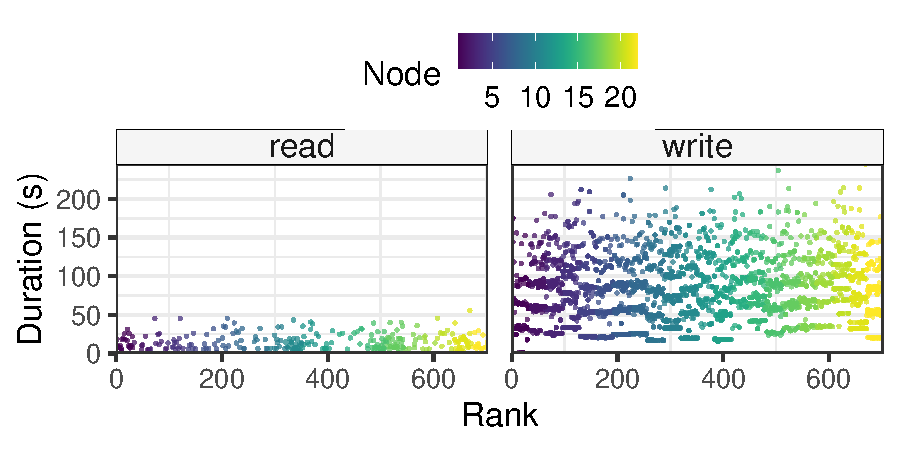
\includegraphics[width=\linewidth]{figs/255653_mpi_io_luster_no_coll_duration.pdf}
        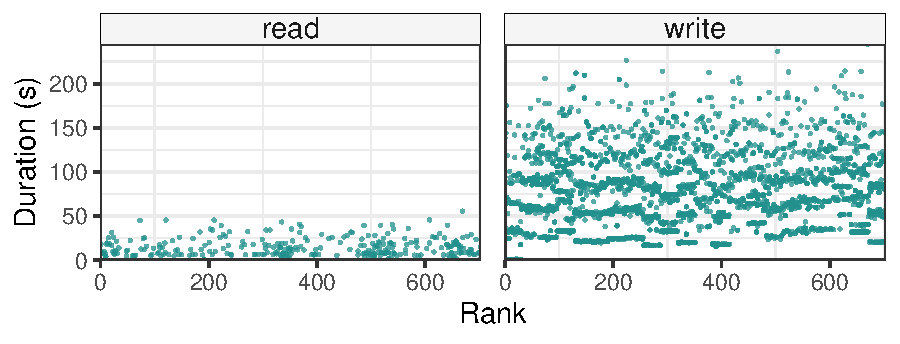
\includegraphics[width=\linewidth]{figs/255653_mpi_io_luster_no_coll_duration_nocolor.pdf}
	\caption{MPI-IO without collective operations. Distribution of reads and writes operations per rank
          and their durations. Some ranks process more/less operations
          and faster/slower.}
	\label{f:mpi_io}
\end{figure}

\begin{figure}
	\centering
	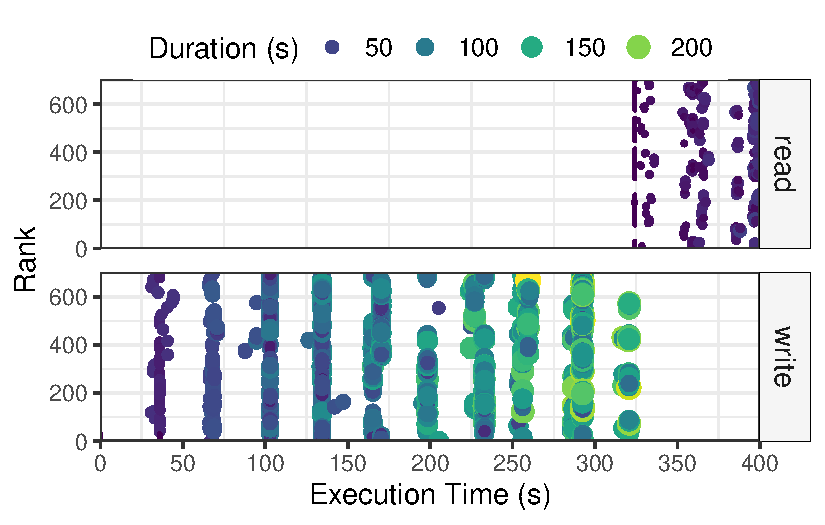
\includegraphics[width=\linewidth]{figs/255653_mpi_io_luster_no_coll_execution2.pdf}
	\caption{MPI-IO without collective operations. Distribution of reads and writes operations
          throughout the execution time, with respective
          durations. The application performs writings during ten
          phases, and then reads at the end.}
	\label{f:mpi_io}
\end{figure}

\begin{figure*}
	\centering
	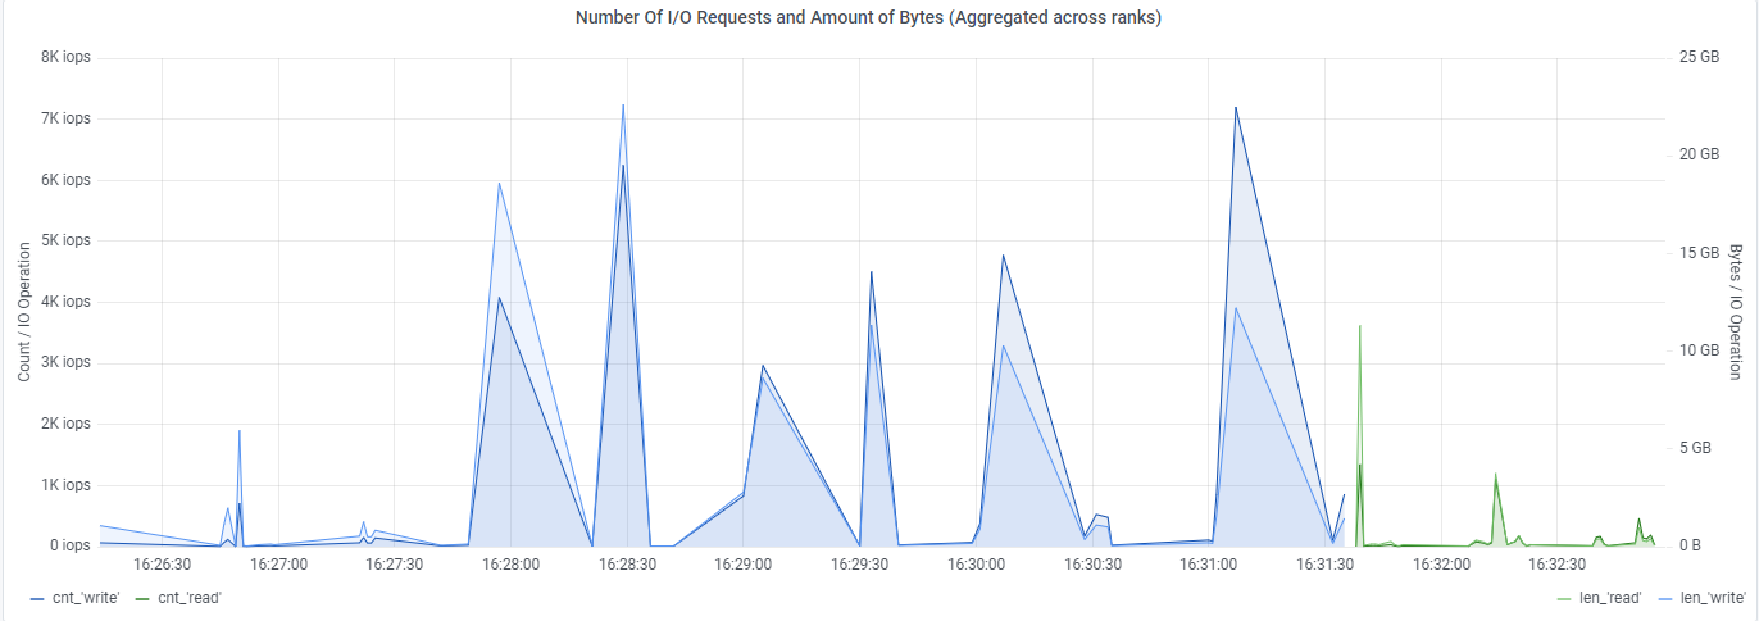
\includegraphics[width=\textwidth]{figs/255653_mpi_io_luster_no_coll.pdf}
	\caption{MPI-IO without collective operations. Graphana visualization using temporal data collected
          with Darshan LDMS}
	\label{f:CSV Header and Output}
      \end{figure*}

 \RED{ADD text about the 3 plots building a narrative how the
   timestamps show valuable insights and we can also see this behavior
 on Grafana.}